\documentclass[12pt,a4paper]{article}
\usepackage{amsmath,amsthm,amsfonts,tikz}
\usepackage[euler-digits]{eulervm}
\usepackage{hyperref}
%%%%%%%%%%%%%%%%%%%%%%%%%%%%%%%%%%%%%%%%%%%%%%%%%%%%%%%%%%%%%%%%%%%%%
\newtheorem{theorem}{Theorem}
\newcommand{\iprod}[1]{\langle#1\rangle}
\newcommand{\vecp}[1]{\boldsymbol{p}}
\newcommand{\hatvecp}{\hat{\boldsymbol{p}}}
\newcommand{\Poly}{\mathbb{P}}
%%%%%%%%%%%%%%%%%%%%%%%%%%%%%%%%%%%%%%%%%%%%%%%%%%%%%%%%%%%%%%%%%%%%%
\title{Notes on Gauss Quadrature for General Weight Functions}
\author{Bill McLean}
\date{\today}
%%%%%%%%%%%%%%%%%%%%%%%%%%%%%%%%%%%%%%%%%%%%%%%%%%%%%%%%%%%%%%%%%%%%%
\begin{document}
\maketitle
\tableofcontents
%%%%%%%%%%%%%%%%%%%%%%%%%%%%%%%%%%%%%%%%%%%%%%%%%%%%%%%%%%%%%%%%%%%%%
\section{Three-term recurrence relation}
Let $\Poly_k$ denote the $(k+1)$-dimensional vector space of real 
polynomials with degree at most~$k$, and denote the 
infinite-dimensional space of all polynomials by~$\Poly$.  Let $\mu$ 
be a positive measure on the real line with the property that, 
$\int f(x)^2\,d\mu(x)=0$~and $f\in\Poly$ then $f=0$.
We can then define an inner product and norm on~$\Poly$  by
\[
\iprod{f,g}=\int f(x)g(x)\,d\mu(x)\quad\text{and}\quad
\|f\|=\sqrt{\iprod{f,f}}.
\]
Using the Gram--Schmidt procedure to orthogonalise the linearly 
independent monomials $1$, $x$, $x^2$, $x^3$, \dots, yields the
polynomial~$p_j(x)$ of degree~$j$ by
\[
p_j(x)=x^j-\sum_{k=0}^{j-1}\frac{\iprod{x^j,p_k}}{\|p_k\|^2}\,p_k(x)
	\quad\text{for $j=0$, $1$, $2$, \dots.}
\]
Therefore, $p_j$ is the unique monic polynomial in~$\Poly_j$ such 
that $p_j\perp\Poly_{j-1}$; in particular,
\begin{equation}\label{eq: orthog}
\iprod{p_j,p_k}=0\quad\text{if $j\ne k$.}
\end{equation}

\begin{theorem}\label{thm: 3 term}
The orthogonal polynomials defined above satisfy the three-term 
recurrence relation
\begin{equation}\label{eq: 3 term pj}
p_j(x)=(x-a_j)p_{j-1}(x)-b_j^2p_{j-2}(x)
	\quad\text{for $j=1$, $2$, $3$, \dots,}
\end{equation}
with $p_0(x)=1$ and $p_{-1}(x)=0$. The coefficients satisfy
\[
a_j=\frac{\iprod{xp_{j-1},p_{j-1}}}{\|p_{j-1}\|^2}
\quad\text{and}\quad
b_j=\frac{\|p_{j-1}\|}{\|p_{j-2}\|},
\]
except that, by convention, we put $b_1=\sqrt{\int d\nu}=\|p_0\|$.
\end{theorem}
\begin{proof}
Since $p_j(x)-xp_{j-1}(x)$ has degree at most~$j-1$, there are 
constants~$c_{jk}$ such that
\[
p_j(x)-xp_{j-1}(x)=\sum_{k=0}^{j-1}c_{jk}p_k(x).
\]
Taking the inner product of both sides with~$p_{j-1}$ and using
the orthogonality property~\eqref{eq: orthog}, we obtain
\[
-\iprod{xp_{j-1},p_{j-1}}=c_{j,j-1}\|p_{j-1}\|^2,
\]
showing that $c_{j,j-1}=-a_j$.  Also, taking the inner product of both
sides with~$p_k$ for $k\le j-3$ gives
\[
c_{jk}\|p_k\|^2=\iprod{p_j-xp_{j-1},p_k}=-\iprod{p_{j-1},xp_k}=0,
\]
so $p_j(x)=(x-a_j)p_{j-1}(x)+c_{j,j-2}p_{j-2}(x)$ and
\[
0=\iprod{p_j,p_{j-2}}=\iprod{xp_{j-1},p_{j-2}}+c_{j,j-2}\|p_{j-2}\|^2.
\]
Finally, 
\begin{align*}
\iprod{xp_{j-1},p_{j-2}}&=\iprod{p_{j-1},xp_{j-2}}
	=\iprod{p_{j-1},p_{j-1}}+\iprod{p_{j-1},xp_{j-2}-p_{j-1}}\\
	&=\|p_{j-1}\|^2+0,
\end{align*}
and therefore $c_{j,j-2}=-\|p_{j-1}\|^2/\|p_{j-2}\|^2=-b_j^2$.
\end{proof}

Recall that the Lagrange interpolation polynomial
\[
\ell_j(x)=\prod_{\substack{k=1\\ k\ne j}}^n\frac{x-x_k}{x_j-x_k}.
\]
has the property that $\ell_j(x_k)=\delta_{jk}$. The zeros of~$p_n$ 
have the following important properties.  

\begin{theorem}
Suppose that $d\mu(x)=w(x)\,dx$ with $w(x)>0$ for $a<x<b$.
(We allow $a=-\infty$ or $b=\infty$.) The orthogonal polynomial has 
only real and simple zeros~$x_j$ in the open interval~$(a,b)$, that 
is,
\[
a<x_1<x_2<\cdots<x_n<b.
\]
\end{theorem}
\begin{proof}
Suppose for a contradiction that $p_n$ has a zero $\alpha+i\beta$ 
with~$\beta\ne0$.  Since $p_n$ has real coefficients, 
the complex conjugate~$\alpha-i\beta$ is also a zero and thus
\[
p_n(x)=\bigl[x-(\alpha+i\beta)\bigr]\bigl[x-(\alpha-i\beta)\bigr]q(x)
	=[(x-\alpha)^2+\beta^2]q(x)
\]
with $n\ge2$~and $q\in\Poly_{n-2}$. Since $p_n\perp\Poly_{n-2}$,
\[
0=\iprod{p_n,q}=\iprod{[(x-\alpha)^2+\beta^2],q}\\
	=\|(x-\alpha)q\|^2+\beta^2\|q\|^2,
\]
implying that $q=0$ and thus $p_n=0$, a contradiction.

Likewise, suppose for a contradiction that $p_n$ has a multiple real 
root~$\alpha$ and write $p_n(x)=(x-\alpha)^2q(x)$ with 
$q\in\Poly_{n-2}$.  Then
\[
0=\iprod{p_n,q}=\iprod{(x-\alpha)^2q,q}=\|(x-\alpha)q\|^2,
\]
again implying that $q=0$ and thus $p_n=0$.  We conclude that $p_n$ 
has only distinct real zeros~$x_j$.

Thus, for $1\le j\le n$,
\[
p_n(x)=\prod_{k=1}^n(x-x_k)=c_j(x-x_j)\ell_j(x)
\quad\text{where}\quad
c_j=\prod_{\substack{k=1\\ k\ne j}}^n(x_j-x_k)\ne0.
\]
Since $\ell_j\in\Poly_{n-1}$ and $p_n\perp\Poly_{n-1}$,
\[
0=\iprod{p_n,\ell_j}=\iprod{c_j(x-x_j)\ell_j,\ell_j}
	=c_j\bigl[(x\ell_j,\ell_j)-x_j\|\ell_j\|^2\bigr],
\]
implying that
\[
x_j=\frac{\iprod{x\ell_j,\ell_j}}{\|\ell_j\|^2}.
\]
By integrating the strict inequalities
\[
a\ell_j(x)^2w(x)<x\ell_j(x)^2w(x)<b\ell_j(x)^2w(x)
	\quad\text{for $a<x<b$,}
\]
we see that $a\|\ell_j\|^2<\iprod{x\ell_j,\ell_j}<b\|\ell_j\|^2$
and therefore $a<x_j<b$, as claimed.
\end{proof}

We denote the ortho\emph{normal} polynomials by
\[
\hat p_j(x)=\frac{p_j(x)}{\|p_j\|},
\]
and find that
\[
b_{j+1}\hat p_j(x)=(x-a_j)\hat p_{j-1}(x)-b_j\hat p_{j-2}(x),
\]
or equivalently,
\begin{equation}\label{eq: 3 term orthog}
b_j\hat p_{j-2}(x)+a_j\hat p_{j-1}(x)+b_{j+1}\hat p_j(x)=xp_{j-1}(x).
\end{equation}

\begin{theorem}[Christoffel--Darboux identity]
\label{thm: Christoffel-Darboux}
The monic orthogonal polynomials satisfy
\[
\frac{1}{b_{n+2}}\sum_{k=0}^n\hat p_k(x)\hat p_k(y)
	=\frac{\hat p_{n+1}(x)\hat p_n(y)-\hat p_n(x)\hat p_{n+1}(y)}{x-y}
	\quad\text{for $x\ne y$.}
\]
\end{theorem}
\begin{proof}
Using \eqref{eq: 3 term orthog}, we see that
\begin{align*}
(x-y)\hat p_{k-1}(x)&\hat p_{k-1}(y)
	=[x\hat p_{k-1}(x)]\hat p_{k-1}(y)
		-\hat p_{k-1}(x)[y\hat p_{k-1}(y)]\\
	&=\bigl[
	b_k\hat p_{k-2}(x)+a_k\hat p_{k-1}(x)+b_{k+1}\hat p_k(x)
	\bigr]\hat p_{k-1}(y)\\
	&\qquad{}-\hat p_{k-1}(x)\bigl[
	b_k\hat p_{k-2}(y)+a_k\hat p_{k-1}(y)+b_{k+1}\hat p_k(y)\bigr]\\
	&=\bigl[b_k\hat p_{k-2}(x)\hat p_{k-1}(y)
		-b_{k+1}\hat p_{k-1}(x)\hat p_k(y)\bigr]\\
	&\qquad{}+\bigl[b_{k+1}\hat p_k(x)\hat p_{k-1}(y)
		-b_k\hat p_{k-1}(x)\hat p_{k-2}(y)\bigr]\\
\end{align*}
and so
\begin{align*}
(x-y)\sum_{k=1}^{n+1}\hat p_{k-1}(x)\hat p_{k-1}(y)
	&=b_1\hat p_{-1}(x)\hat p_0(y)-b_{n+2}\hat p_n(x)\hat p_{n+1}(y)\\
	&\qquad{}+b_{n+2}\hat p_{n+1}(x)\hat p_n(y)
		-b_1\hat p_0(x)\hat p_{-1}(y).
\end{align*}
\end{proof}


\subsection{Legendre polynomials}
The Legendre polynomials have the orthogonality property
\begin{equation}\label{eq: legendre orthog}
\int_{-1}^1 P_k(x)P_l(x)\,dx=\frac{2\delta_{kl}}{2k+1}
\end{equation}
and the 3-term recurrence relation is
\begin{equation}\label{eq: legendre 3 term}
kP_k(x)=(2k-1)xP_{k-1}(x)-(k-1)P_{k-2}(x).
\end{equation}
The normalised Legendre polynomials are
\[
\hat P_k(x)=\frac{P_k(x)}{\|P_k\|}=\biggl(\frac{2k+1}{2}\biggr)^{1/2}
	P_k(x),
\]
and thus
\begin{multline*}
k\biggl(\frac{2}{2k+1}\biggr)^{1/2}\hat P_k(x)
	=(2k-1)\biggl(\frac{2}{2k-1}\biggr)^{1/2}x\hat P_{k-1}(x)\\
	-(k-1)\biggl(\frac{2}{2k-3}\biggr)^{1/2}\hat P_{k-2}(x),
\end{multline*}
or equivalently,
\[
\frac{k\hat P_k(x)}{\sqrt{2k+1}}=\sqrt{2k-1}\,x\hat P_{k-1}(x)
	-\frac{k-1}{\sqrt{2k-3}}\,\hat P_{k-2}(x).
\]
Thus, the Legendre polynomials satisfy
\[
b_{k+1}\hat P_k(x)=(x-a_k)\hat P_{k-1}(x)-b_k\hat P_{k-2}(x)
\]
where
\[
a_k=0\quad\text{and}\quad b_k=\frac{k-1}{\sqrt{(2k-1)(2k-3)}},
\]
except that $b_1=\sqrt{\int_{-1}^1\,dx}=\sqrt{2}$.

\section{Gauss quadrature}
We now consider a quadrature rule
\begin{equation}\label{eq: Qf}
Qf=\sum_{j=1}^n w_jf(x_j)
\end{equation}
and its associated error functional
\[
Ef=\int f(x)\,d\mu(x)-\sum_{j=1}^n w_jf(x_j).
\]

\begin{theorem}\label{thm: Gauss rule}
For each $n\ge1$ there exists a unique quadrature rule~\eqref{eq: Qf}
such that
\begin{equation}\label{eq: dop 2n-1}
Ef=0\quad\text{for all $f\in\Poly_{2n-1}$.}
\end{equation}
This rule has has as its integration points $x_1$, $x_2$, \dots, 
$x_n$ the zeros of~$p_n$, that is,
\[
p_n(x_j)=0\quad\text{for $1\le j\le n$,}
\]
and as its weights the numbers
\begin{equation}\label{eq: Gauss weights}
w_j=\iprod{\ell_j,1}=\int\ell_j(x)\,d\mu(x)>0
	\quad\text{for $1\le j\le n$,}
\end{equation}
where $\ell_j$ is the $j$th Lagrange interpolation polynomial:
\[
\ell_j(x)=\prod_{\substack{k=1\\ k\ne j}}\frac{x-x_k}{x_j-x_k}.
\]
\end{theorem}
\begin{proof}
Let $x_1$, $x_2$, \dots, $x_n$ be the zeros of~$p_n$, and define
$w_j=\iprod{\ell_j,1}$.  Given $f\in\Poly_{2n-1}$, let $q$~and $r$ 
denote the quotient and remainder when $f$ is divided by~$p_n$, that 
is,
\[
f(x)=p_n(x)q(x)+r(x)\quad\text{with $r\in\Poly_{n-1}$.}
\]
Since $p_n(x_j)=0$ it follows that $f(x_j)=r(x_j)$ and so
\[
r(x)=\sum_{j=1}^n f(x_j)\ell(x),
\]
and since $q\in\Poly_{n-1}$ and $p_n$ is orthogonal to~$\Poly_{n-1}$,
\begin{multline*}
\int f(x)\,d\mu(x)=\int q(x)p_n(x)\,d\mu(x)+\int r(x)\,d\mu(x)\\
	=\iprod{q,p_n}+\sum_{j=1}^n f(x_j)\int\ell_j(x)\,d\mu(x)
	=0+\sum_{j=1}^n f(x_j)\iprod{\ell_j,1}=Qf,
\end{multline*}
showing that $Ef=0$.  

To prove uniqueness, let $Q$ be any quadrature rule~\eqref{eq: Qf} 
satisfying \eqref{eq: dop 2n-1}.  Consider the 
polynomial~$f\in\Poly_n$ defined by
\[
f(x)=(x-x_1)(x-x_2)\cdots(x-x_n).
\]
If $0\le k\le n-1$ then $x^kf(x)\in\Poly_{2n-1}$ so
\[
\iprod{x^k,f}=\int x^kf(x)\,d\mu(x)=\sum_{j=1}^n w_jx_j^kf(x_j)=0.
\]
Hence, $f\perp\Poly_{n-1}$, and since $f$ is monic it follows that 
$f=p_n$ by the uniqueness of the orthogonal polynomials.  Therefore,
the $x_j$ are the zeros of~$p_n$, and moreover
\[
w_j=\sum_{k=1}^nw_k\ell_j(x_k)=\int\ell_k(x)\,d\mu(x)=\iprod{\ell_j,1}
\]
since $\ell_j\in\Poly_{n-1}$.  In fact, $\ell_j^2\in\Poly_{2n-2}$ so
\[
w_j=\sum_{k=1}^nw_k\ell_j(x_k)^2=\int\ell_j(x)^2\,d\mu(x)
	=\|\ell_j\|^2>0,
\]
and the weights satisfy~\eqref{eq: Gauss weights}.
\end{proof}

The quadrature in the theorem above is called the $n$-point Gauss 
rule generated by the positive measure~$\mu$.

Defining
\[
T_n=\begin{bmatrix}
a_1&b_2   &       &       &\\
b_2&a_2   &b_3    &       &\\
   &\ddots&\ddots &\ddots &\\
   &      &b_{n-1}&a_{n-1}&b_n\\
   &      &       &b_n    &a_n
\end{bmatrix}
\quad\text{and}\quad
\hatvecp_n(x)=\begin{bmatrix}
	\hat p_0(x)\\ \hat p_1(x)\\ \vdots\\ \hat p_{n-1}(x)
\end{bmatrix},
\]
the equations~\eqref{eq: 3 term orthog} for $0\le j\le n-1$ are 
equivalent to
\begin{equation}\label{eq: matrix 3 term orthog}
T_n\hatvecp_n(x)+b_{n+1}\hat p_n(x)\boldsymbol{e}_n=x\hatvecp_n(x).
\end{equation}
The points~$x_j$ and weights~$w_j$ may be computed by solving an 
eigenproblem for the \emph{Jacobi matrix}~$T_n$.

\begin{theorem}
The eigenvalues of~$T_n$ are the points $x_1$, $x_2$, \dots, $x_n$
of the associated Gauss quadrature rule.  Moreover, for~$1\le j\le n$,
if
\[
\boldsymbol{v}_j=\begin{bmatrix}v_{1j}\\ v_{2j}\\ \vdots\\ v_{nj}
\end{bmatrix}
\]
denotes the eigenvector of~$T_n$ satisfying
\[
T_n\boldsymbol{v}_j=x_j\boldsymbol{v}_j
\quad\text{and}\quad
v_{1j}=\frac{1}{b_1},
\]
then the weight~$w_j$ corresponding to the $j$th Gauss point~$x_j$ 
is given by
\[
\frac{1}{w_j}=\sum_{k=1}^n(v_{kj})^2.
\]
\end{theorem}
\begin{proof}
We see at once from~\eqref{eq: matrix 3 term orthog} that 
$T_n\hatvecp_n(x)=x\hatvecp_n(x)$ iff $p_n(x_j)=0$, so the
eigenvalues~$x_j$ of~$T_n$ coincide with zeros of~$p_n$ which,
by Theorem~\ref{thm: Gauss rule}, coincide with the Gauss points.  
Moreover, $\boldsymbol{v}_j=\hatvecp_n(x_j)$ is the eigenvector 
of~$T_n$ that corresponds to the eigenvalue~$x_j$ and is scaled in 
such a way that $v_{1k}=\hat p_0(x_j)=1/\|p_0\|=1/b_1$.

Since $p_n$ is monic with zeros $x_1$, $x_2$, \dots, $x_n$,
\[
p_n(x)=\prod_{j=1}^n(x-x_j)
\qquad\text{and thus}\qquad
p_n'(x)=\sum_{j=1}^n\prod_{\substack{k=1\\ k\ne j}}^n(x-x_k).
\]
In particular
\[
p_n'(x_j)=\prod_{\substack{k=1\\ k\ne j}}^n(x_j-x_k),
\]
showing that
\[
p_n(x)=p_n'(x_j)(x-x_j)\ell_j(x)\quad\text{where}\quad
\ell_j(x)=\prod_{\substack{k-1\\ k\ne j}}\frac{x-x_k}{x_j-x_k}.
\]
Hence, $\hat p_n(x)=\hat p_n'(x_j)(x-x_j)\ell_j(x)$ and so
\begin{equation}\label{eq: w_j}
w_j=\iprod{\ell_j,1}=\frac{1}{\hat p_n'(x_j)}
	\int_a^b\frac{\hat p_n(x)}{x-x_j}\,w(x)\,dx
\end{equation}
Putting $y=x_j$ in the Christoffel--Darboux identity of 
Theorem~\ref{thm: Christoffel-Darboux} gives
\[
\frac{1}{b_{n+1}}\sum_{k=0}^n\hat p_k(x)\hat p_k(x_j)
	=-\frac{\hat p_n(x)}{x-x_j}\,\hat p_{n+1}(x_j)
\]
and after taking the inner product of both sides with~$p_0(x)=1$
we obtain
\[
\frac{1}{b_{n+2}}\sum_{k=0}^n\iprod{\hat p_k,p_0}\hat p_k(x_j)
	=-\hat p_{n+1}(x_j)\int_a^b\frac{\hat p_n(x)}{x-x_j}\,w(x)\,dx.
\]
Here, $\iprod{\hat p_k,p_0}=0$ for~$k\ge1$ and 
$\iprod{\hat p_0,p_0}=\iprod{p_0,p_0}/\|p_0\|=\|p_0\|$, so 
by~\eqref{eq: w_j}
\[
\frac{1}{b_{n+2}}=-\hat p_{n+1}(x_j)\hat p_n'(x_j)w_j.
\]
The Christoffel--Darboux identity also gives
\begin{align*}
\frac{1}{b_{n+2}}\sum_{k=0}^n\hat p_k(x_j)^2
&=\lim_{y\to x_j}\frac{1}{b_{n+2}}\sum_{k=0}^n
	\hat p_k(x_j)\hat p_k(y)
=\lim_{y\to x_j}\frac{\hat p_{n+1}(x_j)\hat p_n(y)}{x_j-y}\\
&=-\hat p_{n+1}(x_j)\lim_{y\to x_j}
	\frac{\hat p_n(y)-\hat p_n(x_j)}{y-x_j}
	=-\hat p_{n+1}(x_j)\hat p_n'(x_j) 
\end{align*}
and therefore
\[
\frac{1}{w_j}=-b_{n+2}\hat p_{n+1}(x_j)\hat p_n'(x_j)
	=\sum_{k=0}^n\hat p_k(x_j)^2=\sum_{k=1}^n(v_{kj})^2,
\]
as claimed.
\end{proof}


\section{The modified Chebyshev algorithm}

Let $q_0$, $q_1$, $q_2$, \dots be a sequence of monic orthogonal 
polynomials generated by a positive measure $\nu$ on the real line.  
Thus, $q_k\in\Poly_k$ is a monic polynomial satisfying 
\[
\int q_k(x)f(x)\,d\nu(x)=0\quad\text{for all $f\in\Poly_{k-1}$.}
\]
In the usual way, we write the three-term recurrence relation as
\begin{equation}\label{eq: 3 term q}
q_k(x)=(x-\alpha_k)q_{k-1}(x)-\beta_k^2 q_{k-2}(x)
	\quad\text{for $k=1$, $2$, $3$, \dots,}
\end{equation}
with
\[
q_0(x)=1\quad\text{and}\quad q_{-1}(x)=0,
\]
adopting the usual convention that $\beta_1=\sqrt{\int d\nu}$.

Suppose that $p_0$, $p_1$, $p_2$, \dots is another sequence of monic 
orthogonal polynomials generated by a positive measure $\mu$ and 
having known coefficients $a_k$~and $b_k$ in the associated 
three-term recurrence relation~\eqref{eq: 3 term pj}; thus
\[
\int p_k(x)f(x)\,d\mu(x)=0\quad\text{for all $f\in\Poly_{k-1}$.}
\]
Following Gautschi~\cite{Gautschi1982}, we consider the case when 
$\alpha_k$~and $\beta_k$ are not known explicitly, but we are able to 
find the generalised moments
\[
\nu_l=\int p_{l-1}(x)\,d\nu(x)\quad\text{for $1\le l\le 2n$.}
\]
The next theorem summarises the modified Chebyshev algorithm for 
computing $\alpha_k$~and $\beta_k$ for $1\le k\le n$.

\begin{figure}
\caption{The dots correspond to the $\sigma_{lk}$ computed in the 
case~$n=5$.  The parallelogram indicates the $\sigma_{lk}$ used in 
the expressions for $\alpha_5$~and $\beta_5$.}
\begin{center}
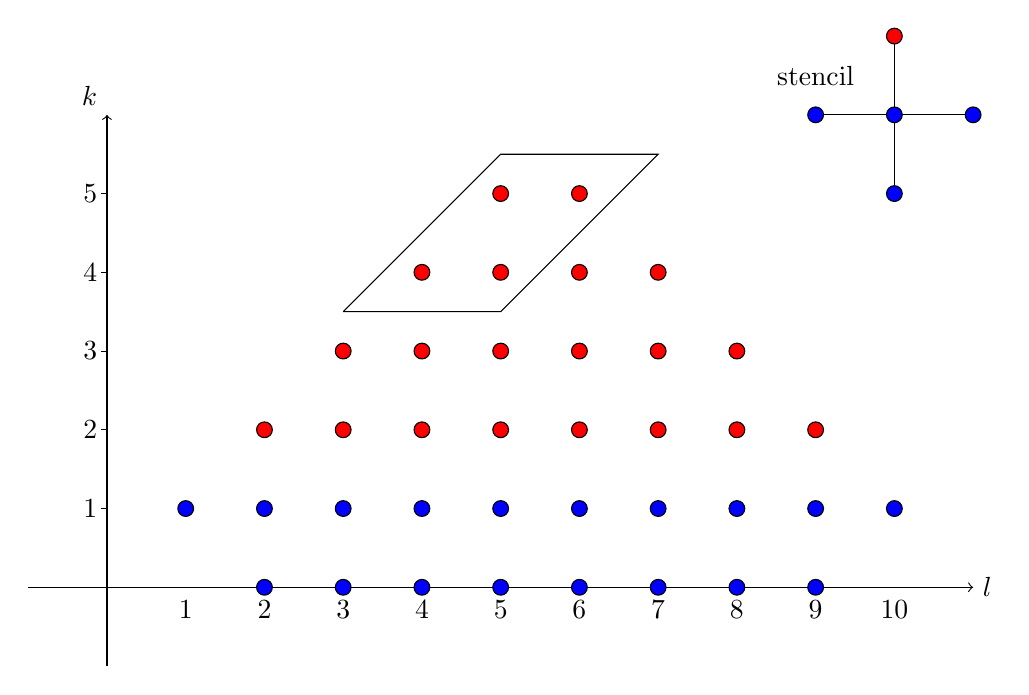
\begin{tikzpicture}[scale=1.0]
\draw[->] (0, -1) -- (0, 6);
\node[above left] at (0, 6) {$k$};
\draw[->] (-1, 0) -- (11, 0);
\node[right] at (11, 0) {$l$};
\foreach \x in {2, 3, ..., 9}
    \draw[fill=blue] (\x, 0) circle(0.10cm);
\foreach \x in {1, 2, ..., 10}
    \draw[fill=blue] (\x, 1) circle(0.10cm);
\foreach \x in {2, 3, ..., 9}
    \draw[fill=red] (\x, 2) circle(0.10cm);
\foreach \x in {3, 4, ..., 8}
    \draw[fill=red] (\x, 3) circle(0.10cm);
\foreach \x in {4, 5, 6, 7}
    \draw[fill=red] (\x, 4) circle(0.10cm);
\foreach \x in {5, 6}
    \draw[fill=red] (\x, 5) circle(0.10cm);
\foreach \y in {1, 2, 3, 4, 5}
    {
    \draw[thin] (-0.075, \y) -- (0, \y);
    \node[left] at (0.0, \y) {$\y$};
    }
\foreach \x in {1, 2, 3, ..., 9, 10}
    \node[below] at (\x, -0.04) {$\x$};
\draw[-] (10, 5) -- (10, 7);
\draw[-] (9, 6) -- (11, 6);
\draw[fill=blue] (9, 6) circle(0.10cm);
\draw[fill=blue] (10, 6) circle(0.10cm);
\draw[fill=blue] (11, 6) circle(0.10cm);
\draw[fill=blue] (10, 5) circle(0.10cm);
\draw[fill=red]  (10, 7) circle(0.10cm);
\node at (9, 6.5) {stencil};
\draw[-] (3.0, 3.5) -- (5.0, 5.5) -- (7.0, 5.5) 
      -- (5.0, 3.5) -- (3.0, 3.5);
\end{tikzpicture}
\end{center}
\end{figure}

\begin{theorem}
The coefficients $\alpha_1$, $\alpha_2$, \dots, $\alpha_n$~and 
$\beta_0$, $\beta_1$, \dots, $\beta_{n-1}$ in the three-term 
recurrence relation~\eqref{eq: 3 term q} can be computed by putting
\[
\begin{aligned}
\sigma_{l,0}&=0&\text{for $2\le l\le 2n-1$},\\
\sigma_{l,1}&=\nu_l&\text{for $1\le l\le2n$},\\
\alpha_1&=a_1+\frac{\nu_2}{\nu_1},\\
\beta_1&=\sqrt{\nu_1},
\end{aligned} 
\]
and, for $k=1$, $2$, \dots, $n-1$ and $k\le l\le2n-k-1$, 
\[
\begin{aligned}
\sigma_{l+1,k+1}&=\sigma_{l+2,k}+(a_{l+1}-\alpha_k)\sigma_{l+1,k}
		+b_{l+1}^2\sigma_{lk}-\beta_k^2\sigma_{l+1,k-1},\\
\alpha_{k+1}&=a_{k+1}+\frac{\sigma_{k+2,k+1}}{\sigma_{k+1,k+1}}
	-\frac{\sigma_{k+1,k}}{\sigma_{kk}},\\
\beta_{k+1}&=\sqrt{\frac{\sigma_{k+1,k+1}}{\sigma_{kk}}}.
\end{aligned}
\]
\end{theorem}
\begin{proof}
It is easily verified that the integrals
\[
\sigma_{lk}=\int p_{l-1}(x)q_{k-1}(x)\,d\nu(x)
\]
satisfy the initial conditions $\sigma_{l,0}=0$~and 
$\sigma_{l,1}=\nu_l$.  In addition, $\sigma_{lk}=0$ if $k>l$. 
For $1\le k\le l$,
\begin{align*}
\sigma_{l+1,k+1}&=\int p_l(x)\bigl[
(x-\alpha_k)q_{k-1}(x)-\beta_k^2q_{k-2}(x)\bigr]\,d\nu(x)\\
	&=\int(x-a_{l+1}+a_{l+1}-\alpha_k)p_l(x)q_{k-1}(x)\,d\nu(x)
		-\beta_k^2\sigma_{l+1,k-1}\\
	&=\int\bigl[(x-a_{l+1})p_l(x)-b_{l+1}^2p_{l-1}(x)\bigr]
		q_{k-1}(x)\,d\nu(x)\\
	&\qquad{}+(a_{l+1}-\alpha_k)\sigma_{l+1,k}
		+b_{l+1}^2\sigma_{lk}-\beta_k^2\sigma_{l+1,k-1}
\end{align*}
so
\[
\sigma_{l+1,k+1}=\sigma_{l+2,k}+(a_{l+1}-\alpha_k)\sigma_{l+1,k}
		+b_{l+1}^2\sigma_{lk}-\beta_k^2\sigma_{l+1,k-1}.
\]

By Theorem~\ref{thm: 3 term},
\[
\alpha_{k+1}=\int xq_k(x)^2\,d\nu(x)\bigg/\int q_k(x)^2\,d\nu(x)
\]
and
\[
\beta_{k+1}^2=\int q_k(x)^2\,d\nu(x)\bigg/\int q_{k-1}(x)^2\,d\nu(x).
\]
Since $q_k(x)-p_k(x)$ has degree at most~$k-1$, the orthogonality 
property of the $q_k$ implies that
\begin{align*}
\int q_k(x)^2\,d\nu(x)&=\int p_k(x)q_k(x)\,d\nu(x)
	+\int\bigl[q_k(x)-p_k(x)\bigr]q_k(x)\,d\nu(x)\\
	&=\sigma_{k+1,k+1}+0,
\end{align*}
so
\[
\beta_{k+1}^2=\frac{\sigma_{k+1,k+1}}{\sigma_{kk}}
	\quad\text{for $k\ge1$,}
	\qquad\text{with $\beta_1^2=\nu_1$.}
\]
Similarly,
\[
\int x q_k(x)^2\,d\nu(x)
	=\int x\bigl[q_k(x)-p_k(x)\bigr]q_k(x)\,d\nu(x)
	+\int xp_k(x)q_k(x)\,d\nu(x),
\]
with
\begin{align*}
\int x&\bigl[q_k(x)-p_k(x)\bigr]q_k(x)\,d\nu(x)
	=\int\bigl[q_k(x)-p_k(x)\bigr](x-\alpha_{k+1})q_k(x)\,d\nu(x)\\
	&\qquad\qquad\qquad\qquad\qquad\qquad{}+\alpha_{k+1}\int 
		\bigl[q_k(x)-p_k(x)\bigr]q_k(x)\,d\nu(x)\\
	&=\int\bigl[q_k(x)-p_k(x)\bigr]
	\bigl[q_{k+1}(x)+\beta_{k+1}^2 q_{k-1}(x)\bigr] 
		\,d\nu(x)+\alpha_{k+1}\times0\\
	&=-\beta_{k+1}^2\sigma_{k+1,k}
	=-\frac{\sigma_{k+1,k+1}}{\sigma_{kk}}\,\sigma_{k+1,k}
\end{align*}
and
\begin{align*}
\int xp_k(x)q_k(x)\,d\nu(x)&=\int\bigl[
	(x-a_{k+1})p_k(x)-b_{k+1}^2p_{k-1}(x)\bigr]q_k(x)\,d\nu(x)\\
	&\qquad{}+\int\bigl[
		a_{k+1}p_k(x)+b_{k+1}^2p_{k-1}(x)\bigr]q_k(x)\,d\nu(x)\\
	&=\int p_{k+1}(x)q_k(x)\,d\nu(x)
		+a_{k+1}\int p_k(x)q_k(x)\,d\nu(x)\\
	&=\sigma_{k+2,k+1}+a_{k+1}\sigma_{k+1,k+1};
\end{align*}
thus,
\[
\alpha_{k+1}=a_{k+1}+\frac{\sigma_{k+2,k+1}}{\sigma_{k+1,k+1}}
	-\frac{\sigma_{k+1,k}}{\sigma_{kk}}
	\quad\text{for $k\ge1$,}
\]
with
\[
\alpha_1=\frac{\sigma_{21}+a_1\sigma_{11}-\beta_1^2\sigma_{1,0}}%
{\sigma_{11}}=a_1+\frac{\sigma_{21}}{\sigma_{11}}
	=a_1+\frac{\nu_2}{\nu_1}.
\]
\end{proof}
%%%%%%%%%%%%%%%%%%%%%%%%%%%%%%%%%%%%%%%%%%%%%%%%%%%%%%%%%%%%%%%%%%%%%
\section{A log weight}
We now consider the example
\[
d\nu(x)=x^\rho\log x^{-1}\,dx\quad\text{for $0<x<1$,}
\]
with $\rho>-1$.  As our known family of orthogonal polynomials we 
use the monic shifted Legendre polynomials,
\[
p_l(x)=\frac{P_l(2x-1)}{C_{l+1}}
\quad\text{where}\quad
C_{l+1}=\binom{2l}{l};
\]
thus
\[
C_l\nu_l=\int_0^1 P_{l-1}(2x-1)x^\rho\log x^{-1}\,dx.
\]
Following \cite{Gautschi1979}, we make the substitution $y=2x-1$
and obtain
\begin{multline*}
C_l\nu_l=\frac{\log 2}{2^{\rho+1}}\int_{-1}^1 
	P_{l-1}(y)(y+1)^\rho\,dy\\
	-\frac{1}{2^{\rho+1}}\int_{-1}^1 
		P_{l-1}(y)(y+1)^\rho\log(y+1)\,dy.
\end{multline*}
It is known that
\[
\int_{-1}^1 P_{l-1}(y)(y+1)^\rho\,dy
	=\frac{2^{\rho+1}\Gamma(\rho+1)^2}%
{\Gamma(\rho+1+l)\Gamma(\rho+2-l)},
\]
and by logarithmic differentiation of this identity with respect 
to~$\rho$, we find that
\begin{multline*}
\int_{-1}^1 P_{l-1}(y)(y+1)^\rho\log(y+1)\,dy
	=\frac{2^{\rho+1}\Gamma(\rho+1)^2}%
{\Gamma(\rho+1+l)\Gamma(\rho+2-l)}\\
	\times\bigl[\log2+2\psi(\rho+1)-\psi(\rho+1+l)-\psi(\rho+2-l)
	\bigr],
\end{multline*}
where $\psi(x)=\Gamma'(x)/\Gamma(x)$ denotes the digamma function.
Thus,
\begin{multline}\label{eq: mu l}
C_l\nu_l
	=\frac{\Gamma(\rho+1)^2}{\Gamma(\rho+1+l)\Gamma(\rho+2-l)} \\
	\times\bigl[\psi(\rho+1+l)+\psi(\rho+2-l)-2\psi(\rho+1)\bigr].
\end{multline}
Using the reflection formulae
\[
\Gamma(1-z)\Gamma(z)=\frac{\pi}{\sin\pi z}
\quad\text{and}\quad
\psi(1-z)=\psi(z)+\pi\cot\pi z,
\]
we find that
\[
\lim_{z\to m}\frac{1}{\Gamma(-z)}=0
\quad\text{and}\quad
\lim_{z\to m}\frac{\psi(-z)}{\Gamma(-z)}=(-1)^{m+1}m!
\]
for $m\in\{0,1,2,\dots\}$.  Thus, if $\rho=r\in\{0,1,2,\dots\}$
then
\[
C_l\nu_l=(-1)^{l-1-r}\,\frac{(r!)^2(l-r-2)!}{(l+r)!}
	\quad\text{for $l\in\{r+2, r+3, r+4, \dots\}$.}
\]
Otherwise, we can use the functional identities
\[
\Gamma(z+1)=z\Gamma(z)\quad\text{and}\quad
\psi(z+1)=\psi(z)+\frac{1}{z}
\]
to simplify \eqref{eq: mu l}.  In fact,
\[
\Gamma(\rho+1)=\rho(\rho-1)\cdots(\rho+2-l)\Gamma(\rho+2-l)
\]
and
\[
\Gamma(\rho+1+l)=(\rho+l)(\rho+l-1)\cdots(\rho+2)(\rho+1)
	\Gamma(\rho+1),
\]
so
\begin{align*}
\frac{\Gamma(\rho+1)^2}{\Gamma(\rho+1+l)\Gamma(\rho+2-l)}
	&=\frac{\rho(\rho-1)\cdots(\rho+2-l)}%
{(\rho+l)(\rho+l-1)\cdots(\rho+2)(\rho+1)}\\
	&=\frac{1}{\rho+1}\prod_{j=1}^{l-1}\frac{\rho+1-j}{\rho+1+j}.
\end{align*}
Moreover,
\[
\psi(\rho+1+l)=\psi(\rho+1)+\frac{1}{\rho+1}+\frac{1}{\rho+2}
	+\cdots+\frac{1}{\rho+l}
\]
and
\[
\psi(\rho+2-l)=\psi(\rho+1)-\frac{1}{\rho}-\frac{1}{\rho-1}
	-\cdots-\frac{1}{\rho-(l-2)},
\]
so
\[
\psi(\rho+1+l)+\psi(\rho+2-l)-2\psi(\rho+1)
	=\frac{1}{\rho+1}+\sum_{j=1}^{l-1}\biggl(\frac{1}{\rho+1+j}
		-\frac{1}{\rho+1-j}\biggr).
\]
Hence,
\begin{equation}\label{eq: Cl nul}
C_l\nu_l=\frac{1}{\rho+1}\biggl[\frac{1}{\rho+1}
	+\sum_{j=1}^{l-1}\biggl(\frac{1}{\rho+1+j}
		-\frac{1}{\rho+1-j}\biggr)\biggr]
	\prod_{k=1}^{l-1}\frac{\rho+1-k}{\rho+1+k},
\end{equation}
and since
\[
C_{l+1}=\frac{(2l)!}{(l!)^2}=\frac{(2l)(2l-1)}{l^2}\,C_l
	=\frac{2(2l-1)}{l}\,C_l
\]
we can compute these coefficients recursively, starting with $C_1=1$.

Choose a non-negative integer~$r$ such that $|\rho-r|$ is as small as 
possible, and define
\[
B_l=\prod_{\substack{k=1\\ k\ne r+1}}^{l-1}\frac{\rho+1-k}{\rho+1+k}
\]
so that
\[
\prod_{k=1}^{l-1}\frac{\rho+1+k}{\rho+1-k}
	=\frac{\rho-r}{\rho+r+2}\,B_l\quad\text{for $l\ge r+2$.}
\]
We can rewrite \eqref{eq: Cl nul} as
\[
C_l\nu_l=\frac{B_l}{1+\rho}\biggl[\frac{1}{1+\rho}+\sum_{j=1}^{l-1}
	\biggl(\frac{1}{\rho+1+j}-\frac{1}{\rho+1-j}\biggr)
		\biggr]\quad\text{for $1\le l\le r+1$,}
\]
with
\begin{multline*}
C_l\nu_l=\frac{B_l}{1+\rho}\,\frac{\rho-r}{\rho+r+2}\biggl[
	\frac{1}{1+\rho}+\sum_{\substack{j=1\\ j\ne r+1}}^{l-1}\biggl(
	\frac{1}{\rho+1+j}-\frac{1}{\rho+1-j}\biggr)\biggr]\\
+\frac{B_l}{1+\rho}\,\frac{1}{\rho+r+2}
	\biggl(\frac{\rho-r}{\rho+r+2}-1\biggr)
		\quad\text{for $l\ge r+2$.}
\end{multline*}


If $\rho=r$ then we can use the formula~\eqref{eq: Cl nul} to compute
$C_l\nu_l$ for $1\le l\le r+1$.  Next, for $l=r+2$,
\[
C_{r+2}\nu_{r+2}=-\,\frac{(r!)^2}{(2r+2)!}=\frac{-1}{2(r+1)}
	\prod_{j=1}^r\frac{j}{2(2j+1)},
\]
and after that we have the recursion
\[
C_{l+1}\nu_{l+1}=-\frac{l-r-1}{l+r+1}\,C_l\nu_l
	\quad\text{for $l\ge r+2$,}
\]
or equivalently,
\[
\nu_{l+1}=-\frac{l-r-1}{l+r+1}\,\frac{l\nu_l}{2(2l-1)}
	\quad\text{for $l\ge r+2$.}
\]



%%%%%%%%%%%%%%%%%%%%%%%%%%%%%%%%%%%%%%%%%%%%%%%%%%%%%%%%%%%%%%%%%%%%%
\bibliographystyle{plain}
\bibliography{notes_refs}
%%%%%%%%%%%%%%%%%%%%%%%%%%%%%%%%%%%%%%%%%%%%%%%%%%%%%%%%%%%%%%%%%%%%%
\end{document}
\endinput
